% TEMPLATE.TEX
%
% Time-stamp: <2013-03-26 11:09 olenz>
%
% This is an extensively documented LaTeX file that shows how to
% produce a good-looking document with current LaTeX (11/2012).
%
% IMPORTANT!
%
%   Some obsolete commands and packages
% ----------|-------------------------------
% obsolete  |     Replacement in LATEX 2ε
% ----------|-------------------------------
%           | local            global/switch
% ----------|-------------------------------
% {\bf ...} | \textbf{...}     \bfseries
%     -     | \emph{...}       \em
% {\it ...} | \textit{...}     \itshape
%     -     | \textmd{...}     \mdseries
% {\rm ...} | \textrm{...}     \rmfamily
% {\sc ...} | \textsc{...}     \scshape
% {\sf ...} | \textsf{...}     \sffamily
% {\sl ...} | \textsl{...}     \slshape
% {\tt ...} | \texttt{...}     \ttfamily
%     -     | \textup{...}     \upshape
%
% DON'T USE \\ TO MAKE LINEBREAKS, INSTEAD JUST LEAVE A BLANK LINE!
%
\RequirePackage[l2tabu,orthodox]{nag} % turn on warnings because of bad style
\documentclass[a4paper,10pt,bibtotoc]{scrartcl}
%
\usepackage[bottom=3.5cm, top=2cm]{geometry}
%%%%%%%%%%%%%%%%%%%%%%%%%%%%%%%%%%%%
% KOMA CLASSES
%%%%%%%%%%%%%%%%%%%%%%%%%%%%%%%%%%%%
%
% The class "scrartcl" is one of the so-called KOMA-classes, a set of
% very well done LaTeX-classes that produce a very European layout
% (e.g. titles with a sans-serif font).
%
% The KOMA classes have extensive documentation that you can access
% via the commands:
%   texdoc scrguide # in German
%   texdoc scrguien # in English
%
%
% The available classes are:
%
% scrartcl - for "articles", typically for up to ~20 pages, the
%            highest level sectioning command is \section
%
% scrreprt - for "reports", typically for up to ~200 pages, the
%            highest level sectioning command is \chapter
%
% scrbook  - for "books", for more than 200 pages, the highest level
%            sectioning command is \part.
%
% USEFUL OPTIONS
%
% a4paper  - Use a4 paper instead of the default american letter
%            format.
%
% 11pt, 12pt, 10pt
%          - Use a font with the given size.
%
% bibtotoc - Add the bibliography to the table of contents
%
% The KOMA-script classes have plenty of options to modify

% This allows to type UTF-8 characters like ä,ö,ü,ß
\usepackage[utf8]{inputenc}

\usepackage[T1]{fontenc}        % Tries to use Postscript Type 1 Fonts for better rendering
\usepackage{lmodern}            % Provides the Latin Modern Font which offers more glyphs than the default Computer Modern
\usepackage[intlimits]{amsmath} % Provides all mathematical commands

\usepackage{hyperref}           % Provides clickable links in the PDF-document for \ref
\usepackage{graphicx}            % Allow you to include images (like graphicx). Usage: \includegraphics{path/to/file}

% Allows to set units
\usepackage[ugly]{units}        % Allows you to type units with correct spacing and font style. Usage: $\unit[100]{m}$ or $\unitfrac[100]{m}{s}$

% Additional packages
\usepackage{url}                % Lets you typeset urls. Usage: \url{http://...}
\usepackage{breakurl}           % Enables linebreaks for urls
\usepackage{xspace}             % Use \xpsace in macros to automatically insert space based on context. Usage: \newcommand{\es}{ESPResSo\xspace}
\usepackage{xcolor}             % Obviously colors. Usage: \color{red} Red text
\usepackage{booktabs}           % Nice rules for tables. Usage \begin{tabular}\toprule ... \midrule ... \bottomrule

% Source code listings
\usepackage{listings}           % Source Code Listings. Usage: \begin{lstlisting}...\end{lstlisting}
\lstloadlanguages{python}
\definecolor{lightpurple}{rgb}{0.8,0.8,1}

\lstset{
stepnumber=1,
numbersep=5pt,
numberstyle=\small\color{black},
basicstyle=\ttfamily,
%keywordstyle=\color{black},
%commentstyle=\color{black},
%stringstyle=\color{black},
frame=single,
tabsize=4,
language = python,
backgroundcolor=\color{black!5}}

\usepackage{float}

\begin{document}

\titlehead{Simulation Methods in Physics I \hfill WS 2019/2010}
\title{Report for Worksheet 6: Finite-Size Scaling and the Ising Model}
\author{Markus Baur and David Beyer}
\date{\today}
%\publishers{Institute for Computational Physics, University of Stuttgart}
\maketitle

\tableofcontents

\section{Speeding up the Simulation}
In this exercise, the skeleton of a Monte Carlo Ising simulation has to be completed. 
Because the simulation stores the configuration of the quadratic Ising lattice in a vector, we first have to implement a mapping scheme from the two indices $i$ and $j$ to the linear index of the vector, this can be done in the following way:
\begin{lstlisting}
int get_linear_index(int i, int j) {
    int index = i * m_l + j;
    return index;
};
\end{lstlisting}
Here, $m_l$ is the number of spins in one direction. 
Since the indices $i$ and $j$ run from $0$ to $m_l-1$, the linear index takes all values between $0$ and $m_l^2 -1$. 
Because the mapping is also linear, it then must be bijective.

In order to initialize the Monte Carlo simulation, all spins $\sigma_{ij}$ have to be assigned a random value $\sigma_{ij}\in\left\{-1,+1\right\}$, this is achieved by the following for-loop:
\begin{lstlisting}
for (auto &i : m_data) {
      i = pow(-1, random_int(2));
      assert((i == 1) or (i == -1));
};
\end{lstlisting}
The random number generator random\_int($n$) is already defined in the given code and produces a random integer in the set $\{0,n-1\}$ according to a uniform distribution.
The assert statement makes sure that every spin can only take values $\pm 1$.
\newpage
\noindent In order to calculate the magnetization of a given spin configuration from scratch, we implemented the following function:
\begin{lstlisting}
void recalculate_magnetization() {
    m_M = std::accumulate(m_data.begin(), m_data.end(), 0);
    assert((m_M >= -m_l * m_l) and (m_M <= m_l * m_l));
};
\end{lstlisting}
This function simply sums all entries of the vector which contains the spin configuration (i.e. it sums the values of all spins). 
The assert statement checks that the absolute value of the magnetization does not exceed $m_l^2$.

We also implemented a function which calculates the total energy of a given spin configuration from scratch:
\begin{lstlisting}
  void recalculate_energy() {
    m_E = 0;
    for (int i = 0; i < m_l; i = i +1 ) {
        for (int j = 0; j < m_l; j = j + 1) {
            m_E += -get(i, j) * (get(i-1, j) +\
            get(i+1, j) + get(i, j-1) + get(i, j+1));
        }
    }
    m_E /= 2;
};
\end{lstlisting}
To calculate the energy, we have to loop over all indices $i$ and $j$ to calculate the interaction energy of all pairs of next neighbours.

In order to make the code faster, we also changed the function set, which allows us to set to value of a given spin $\sigma_{ij}$:
\begin{lstlisting}
void set(int i, int j, int v) {
    assert((v == 1) or (v == -1));
    int _i = mod(i, m_l);
    int _j = mod(j, m_l);
    assert(_i >= 0 and _i < m_l);
    assert(_j >= 0 and _j < m_l);
    if (m_data[get_linear_index(_i, _j)] == -1*v)
    {
        m_M += 2*v;
        m_E += 2.0 * get(i, j) * (get(i-1, j) + get(i+1, j) +\
        get(i, j-1) + get(i, j+1));
    }
    m_data[get_linear_index(_i, _j)] = v;
};
\end{lstlisting}
Using an if-loop, the magnetization and energy get updated if a spin gets changed.

Finally, we implemented a function which allows us to sample the configuration space of the Ising model according to the Metropolis algorithm. 
The function try\_flip decides if a given spin $\sigma_{ij}$ is flipped using the Metropolis criterion:
\begin{lstlisting}
bool try_flip(int i, int j) {
    double energy_difference = -2.0 * get(i, j) * (get(i-1, j) +\
    get(i+1, j) + get(i, j-1) + get(i, j+1));
    if (random_double() <= std::min(1.0,\
    exp(m_beta * energy_difference)))
    {
        set(i, j, -1 * get(i, j));
        return true;
    }
    else
    {
        return false;
    }
};
\end{lstlisting}
If the spin gets flipped, the energy and magnetization are automatically updated as well.
The function returns a Boolean variable whose value depends on the acceptance of the proposed new state.

In order to perform a Metropolis-Monte-Carlo step for a random spin, we implemented the function try\_random\_flip(), which simply executes the function try\_flip(), which was described above, for two random integers in the set $\{0,m_l-1\}$ and returns a Boolean variable depending on the acceptance of the proposed step.
\begin{lstlisting}
bool try_random_flip() {
    return try_flip(random_int(m_l), random_int(m_l));
};
\end{lstlisting}
Furthermore, we also implemented a function try\_many\_random\_flips($n$) which simply performs $n$ Metropolis-Monte-Carlo steps for randomly chosen spins, this is achieved by a simple for-loop:
\begin{lstlisting}
void try_many_random_flips(int n) {
    for (int i = 0; i < n; i = i + 1) {
        try_random_flip();
    }
}
\end{lstlisting}
Using the provided test script, we could verify that the code functions correctly.


\section{Determining Equilibrium Values and Errors}
The code for this section can be found in the file ex3.py.

In order to obtain equilibrium values of the observables (magnetization and energy), we ran simulations for $L=16,64$ and different temperatures. 
To determine the errors of our simulations, we used the code provided in the script ising.py.
Furthermore, we also compare our measurement to the exact summation for $L=4$ and the analytical result for the magnetization in an infinite system.
For all simulations in this section, we first ran 100000000 initial Monte Carlo steps which were not recorded, then we ran another 100000000 steps of which we stored every 1000th.

The simulation results are shown in \autoref{fig:figex3_1} -- \autoref{fig:figex3_4}. 
By comparing the different curves for the magnetization, we can easily see, that they approximate the analytical curve for an infinite system better for larger $L$, as $L$ increases, the curves become steeper near the critical temperature.
However we will never get the nonanalytical part at the critical temperature for a finite system. 
Similary, we observe that the slope of the energy as a function of temperature increases as $L$ becomes larger.
In this case also however, the function is still analytic for a finite system.


\begin{figure}[H]
	\centering
	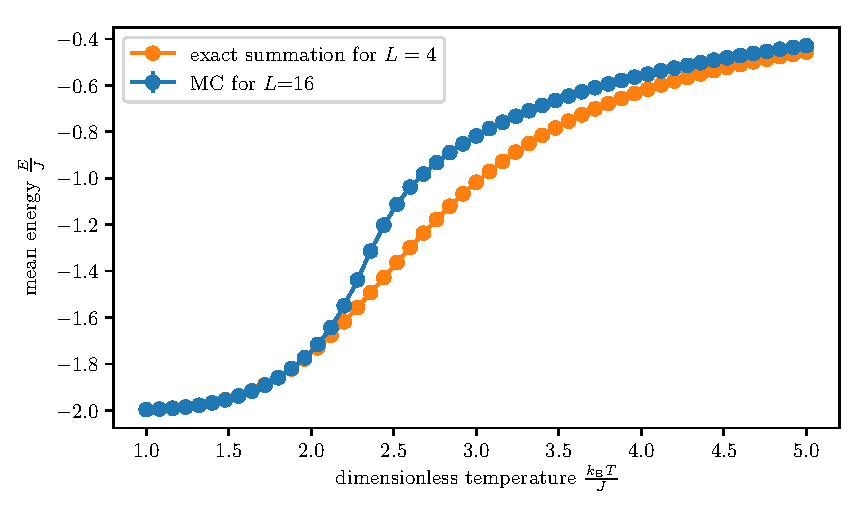
\includegraphics[width=\linewidth]{e16.pdf}
	\caption{Plot of the mean energy per spin as a function of temperature. The plot shows the exact result for a system with $L=4$ and a Monte-Carlo simulation for $L=16$ (with errorbars).}
	\label{fig:figex3_1}
	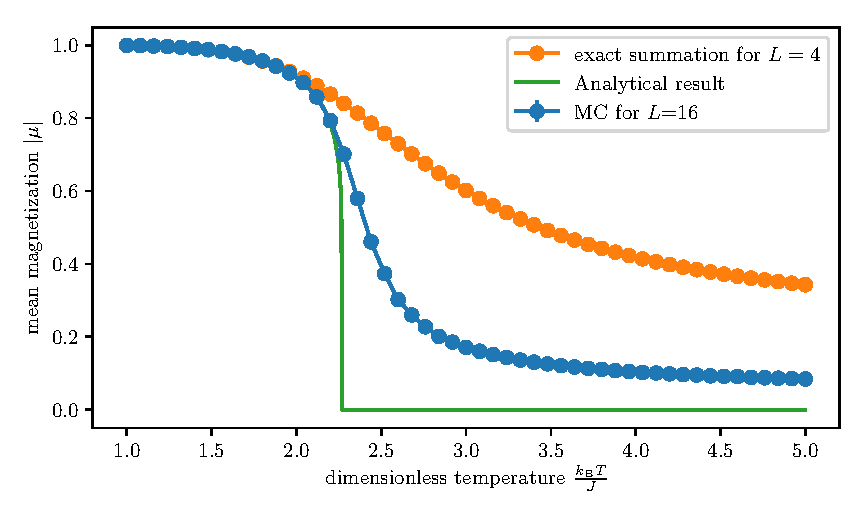
\includegraphics[width=\linewidth]{m16.pdf}
	\caption{Plot of the mean absolute magnetization as a function of temperature. The plot shows the exact result for a system with $L=4$ and a Monte-Carlo simulation for $L=16$ (with errorbars). Furthermore, the analytical result for an infinte system is shown.}
	\label{fig:figex3_2}
\end{figure}

\begin{figure}[H]
	\centering
	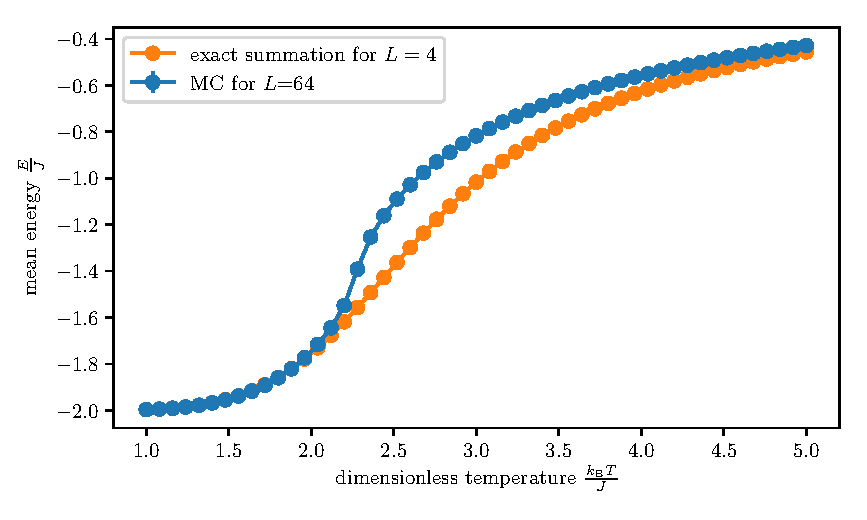
\includegraphics[width=\linewidth]{e64.pdf}
	\caption{Plot of the mean energy per spin as a function of temperature. The plot shows the exact result for a system with $L=4$ and a Monte-Carlo simulation for $L=16$ (with errorbars).}
	\label{fig:figex3_3}
	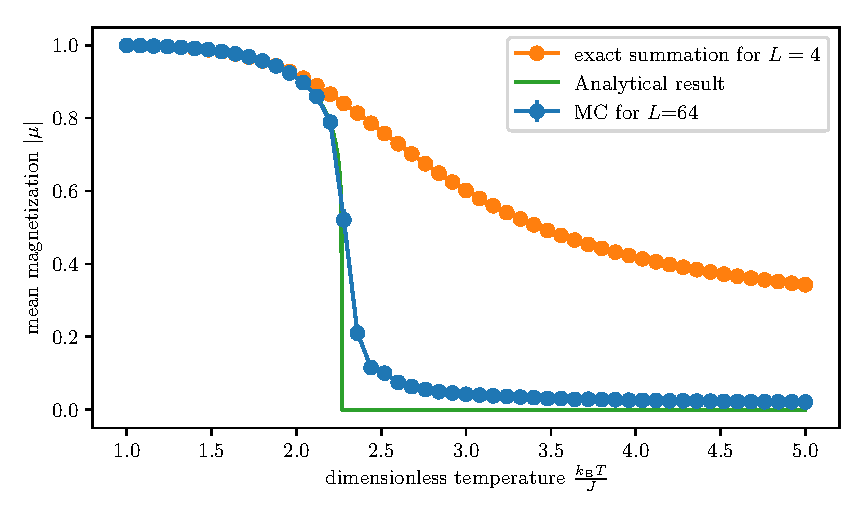
\includegraphics[width=\linewidth]{m64.pdf}
	\caption{Plot of the mean absolute magnetization as a function of temperature. The plot shows the exact result for a system with $L=4$ and a Monte-Carlo simulation for $L=16$ (with errorbars). Furthermore, the analytical result for an infinte system is shown.}
	\label{fig:figex3_4}
\end{figure}

\newpage
\section{Finite Size Scaling}
The code for the following tasks can be found in the files ex4\_1.py, ex4\_2.py, ex4\_3.py and ex4\_3\_analyze.py.
\subsection{Determining $T_\mathrm{c}$}
In order to calculate the Binder parameter for a given Monte-Carlo series, we implemented the following function:
\begin{lstlisting}
def binder_parameter(mu):
    ret = 1 - np.average(mu**4)/(3 * np.average(mu**2)**2)
    return ret
\end{lstlisting}
To perform a Monte-Carlo simulation for different system sizes and temperatures, we used this nested for-loop:
\begin{lstlisting}
for L in Ls:
    U_temp = []
    for T in tqdm(Ts):
        I = cising.IsingModel(1.0/T, L)
        Ms = []
        I.try_many_random_flips(N_initial)
        for i in range(N_MC):
            I.try_random_flip()
            Ms.append(I.magnetization())
        U_temp.append(binder_parameter(np.array(Ms)))
        
    U[L] = U_temp
\end{lstlisting}
$U$ is simply a dictionary in which we store $U(T)$ for the different system sizes. 
In order to reach equilibrium, we first perform N\_initial Monte-Carlo steps which we do not record.
Then, we perform another N\_MC Monte-Carlo steps which we use to calculate the Binder parameter for a given temperature.

Once we have obtained $U(T)$ for different system sizes $L$, we have to find the points where the different curves intersect.
We solved this problem in the following way:
\begin{lstlisting}
for i,j in itertools.combinations(Ls, 2):
    f1 = interpolate.interp1d(Ts, np.array(U[i])-np.array(U[j]),\\
    kind='quadratic')    
    T_intersection.append(optimize.bisect(f1,2.0, 2.4))
\end{lstlisting}
This for-loop runs over all possible combinations of two different system sizes (the order does not matter).
Inside the loop, an interpolation of the differnece of two of the curves is performed using scipy.interpolate.interpi1d.
The intersection of these two curves can then be easily found by finding the root of this interpolated function, this is achieved using scipy.optimize.bisect over the given interval $[2.0,2.4]$.
Once the intersection has been determined, it is added to a list which is averaged at the end of the program, this gives an approximation of the critical temperature.

To determine the Binder parameter and critical temperature, we ran simulations with N\_initial = 100000000 and N\_MC = 100000000 steps.
The value we determined for the critical temperature was
\begin{align}
T_\mathrm{c, Binder} \approx 2.265
\end{align}
which is quite close to the exact value of
\begin{align}
T_\mathrm{c} = \frac{2}{\ln\left(1+\sqrt{2}\right)}\approx 2.2692.
\end{align}
\autoref{fig:figex4_1} shows a plot of the Binder parameter as a function of the temperature $T$.

\begin{figure}[H]
	\centering
	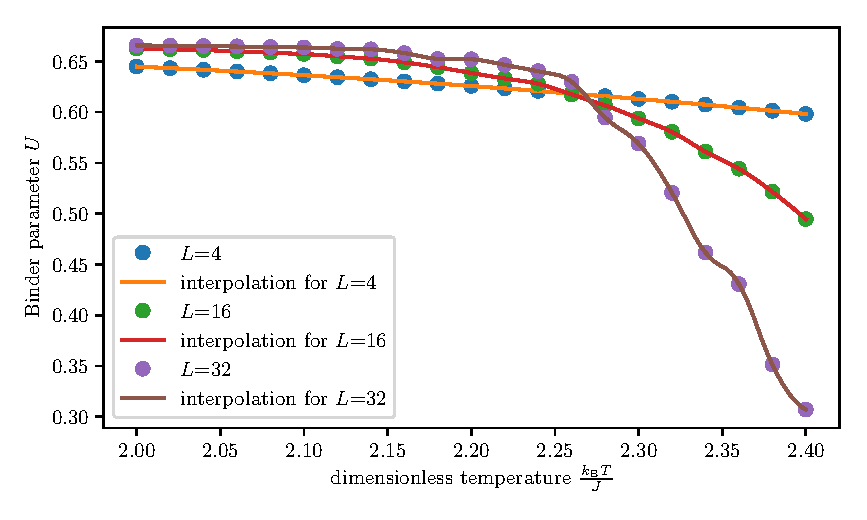
\includegraphics[width=\linewidth]{binder.pdf}
	\caption{Plot of the Binder parameter $U$ as a function of $T$ for different system sizes. The different curves intersect approximately at the critical temperature $T_\mathrm{c}$.}
	\label{fig:figex4_1}
\end{figure}

\subsection{Estimating $\beta_m$}
We now perform simulations for different system sizes $L$ at the critical temperature $T_\mathrm{c}$.
Because we have an approximate value of the critical temperature (determined in the preceding section) as well as the exact value, we might as well compare the results for both of them.
In order to determine critical exponent $\beta_m$, we make use of the scaling behaviour of the magnetization near the critical temperature.
From the lecture it is known that we have
\begin{align}
m\sim L^{-\beta_m/\nu}\tilde{f}\left(tL^{1/\nu}\right).
\end{align}
At the critical temperature ($t=0$), the scaling function $\tilde{f}$ is constant, so we have
\begin{align}
m\sim L^{-\beta_m/\nu}.
\end{align}
This means that we can determine the exponent $\beta_m/\nu$ by taking the logarithm on both sides and fitting a linear function. 
Since we know that $\nu=-1$ for the 2D Ising model, we can then determine the value of the critical exponent $\beta_m$. 

We performed Monte Carlo simulations at both the exact critical temperature as well as at the numerically determined approximate critical temperature for the system sizes $L=8,16,32,64,128$.
The results are plotted in \autoref{fig:figex4_2_1} and \autoref{fig:figex4_2_2}.
For the simulation at the exact critical temperature $T_\mathrm{c}$ we get
\begin{align}
\beta_m\approx -0.1520.
\end{align}
For the simulation at the numerically determined approximate critical temperature $T_\mathrm{c,Binder}$ we get
\begin{align}
\beta_m\approx -0.0840.
\end{align}
We can see that the value of $\beta_m$ depends quite strongly on the value of the critical temperature $T_\mathrm{c}$.
As a comparison, the exact (analytical) result is
\begin{align}
\beta_{m,\mathrm{exact}} = \frac{1}{8} = -0.125.
\end{align}


\begin{figure}[H]
	\centering
	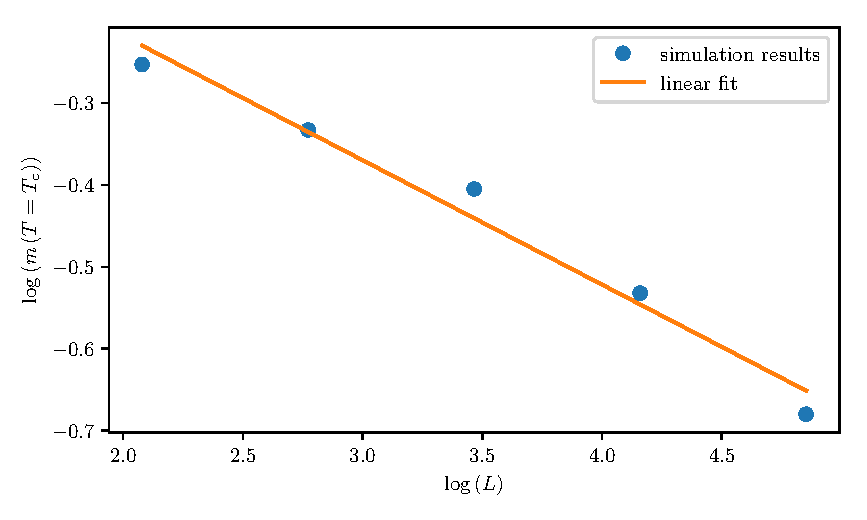
\includegraphics[width=\linewidth]{beta_fit_exact.pdf}
	\caption{Double logarithmic plot of the magnetization as a function of the system size $L$ at the exact critical temperature $T_\mathrm{c} = \frac{2}{\ln\left(1+\sqrt{2}\right)}$ and linear fit.}
	\label{fig:figex4_2_1}
	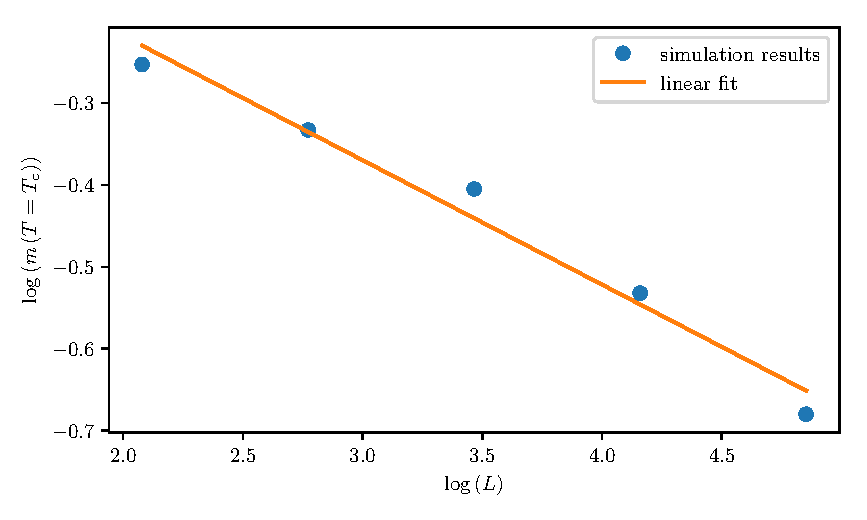
\includegraphics[width=\linewidth]{beta_fit_exact.pdf}
	\caption{Double logarithmic plot of the magnetization as a function of the system size $L$ at the approximate critical temperature (numerically determined) $TT_\mathrm{c, Binder} \approx 2.265$ and linear fit.}
	\label{fig:figex4_2_2}
\end{figure}

\newpage
\subsection{The Master Curve}
The plots \autoref{fig:figex4_3_1} -- \autoref{fig:figex4_3_6} show the master curve for different values of the exponent $a$.
We can see that the plot for the estimated value of $\beta_m=-0.0840=-a$ looks quite well around the critical temperature. 
The plots for $\beta_m=-0.125=-a$ and $\beta_m=-0.152=-a$ fit even better.

\begin{figure}[H]
	\centering
	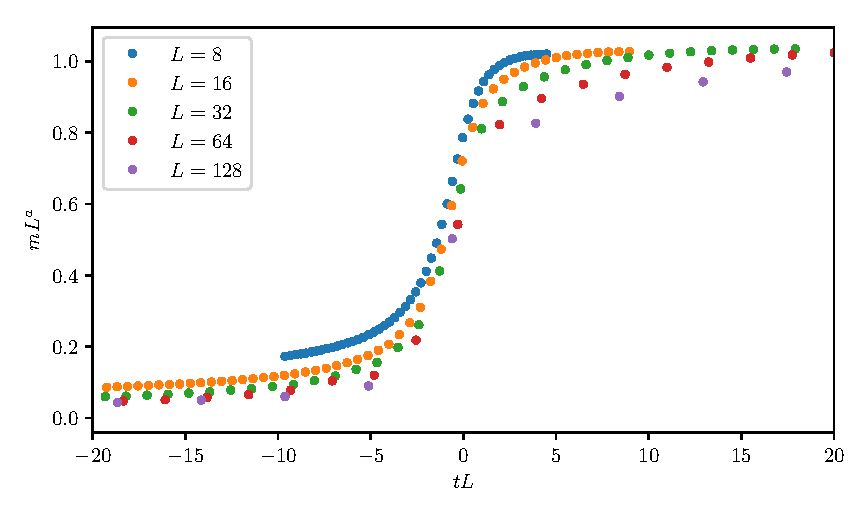
\includegraphics[width=\linewidth]{a001.pdf}
	\caption{Plot of the master curve for $a=0.01$.}
	\label{fig:figex4_3_1}
\end{figure}

\begin{figure}[H]
	\centering
	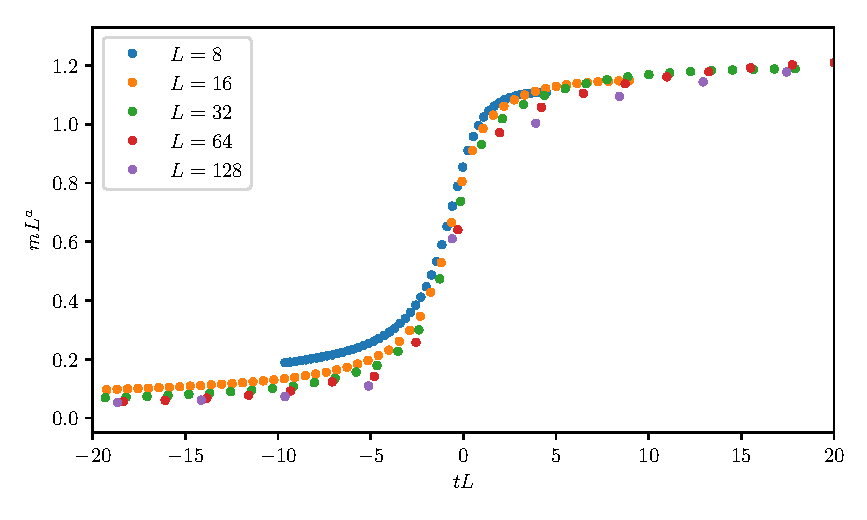
\includegraphics[width=\linewidth]{a005.pdf}
	\caption{Plot of the master curve for $a=0.05$.}
	\label{fig:figex4_3_2}
\end{figure}

\begin{figure}[H]
	\centering
	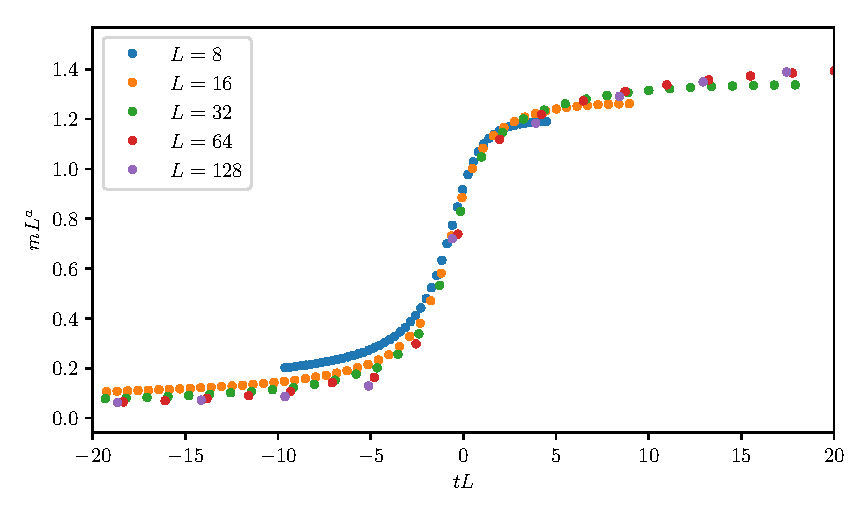
\includegraphics[width=\linewidth]{a0840.pdf}
	\caption{Plot of the master curve for $a=0.0840$.}
	\label{fig:figex4_3_3}
\end{figure}

\begin{figure}[H]
	\centering
	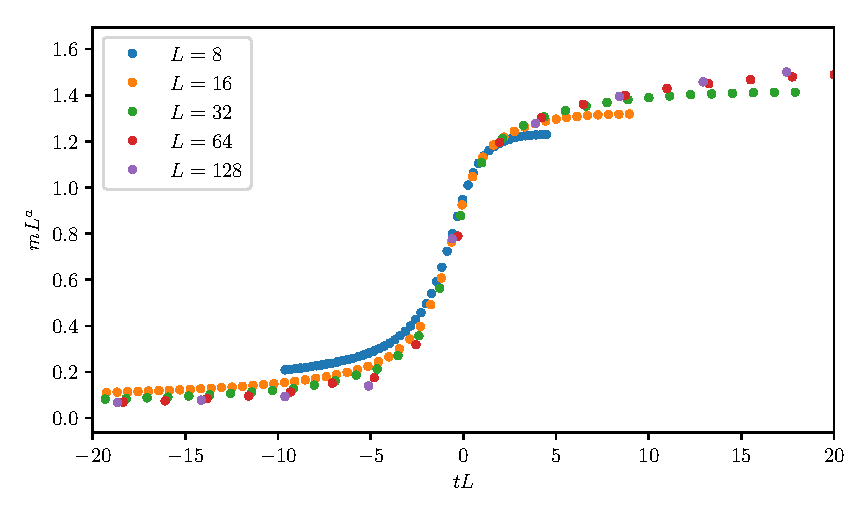
\includegraphics[width=\linewidth]{a01.pdf}
	\caption{Plot of the master curve for $a=0.1$.}
	\label{fig:figex4_3_4}
\end{figure}

\begin{figure}[H]
	\centering
	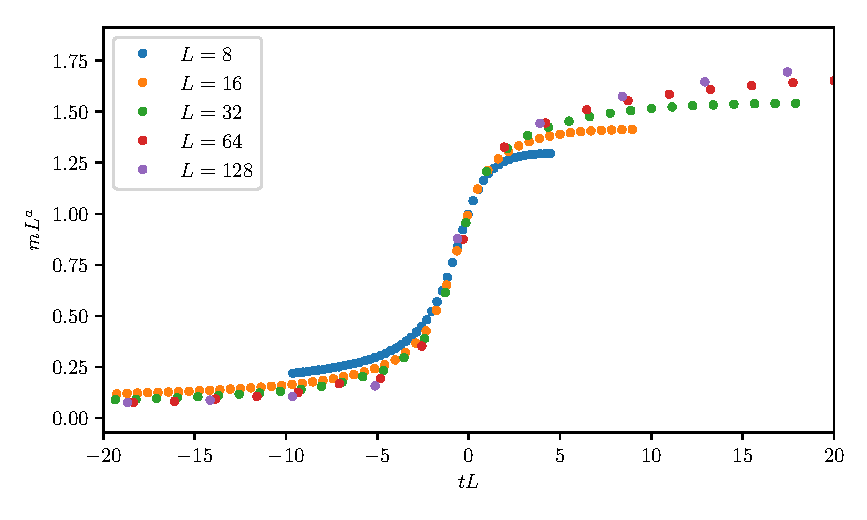
\includegraphics[width=\linewidth]{a125.pdf}
	\caption{Plot of the master curve for $a=0.125$.}
	\label{fig:figex4_3_5}
\end{figure}

\begin{figure}[H]
	\centering
	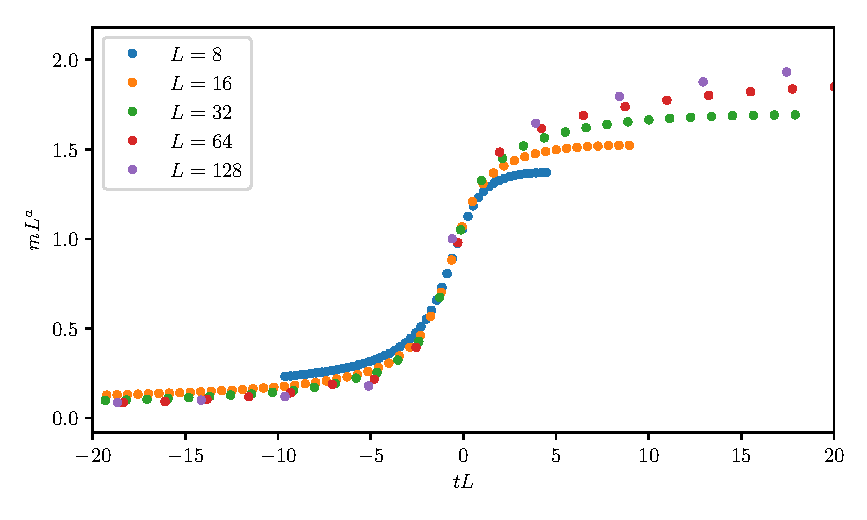
\includegraphics[width=\linewidth]{a1520.pdf}
	\caption{Plot of the master curve for $a=0.152$.}
	\label{fig:figex4_3_6}
\end{figure}



\newpage
\section{Calculating the Magnetic Susceptibility from Fluctuating Magnetization}
The Hamiltonian for the Ising model in an external magnetic field $B$ is given by
\begin{align}
H = -J\sum_{\langle i, j\rangle} \sigma_i\sigma_j - B\sum_{i} \sigma_i.
\end{align}
The units have been chosen in such a way that the spins are dimensionless. The first sum runs over all pairs of neighbouring spins while the second sum runs over all spins. In the canonical ensemble, the mean magnetization $m$ at the inverse temperature $\beta$ is given by
\begin{align}
m = \left\langle\frac{1}{L^2}\sum_{i}\sigma_i\right\rangle = \sum_{\left\{\sigma_i\right\}}\frac{e^{-\beta H\left(\left\{\sigma_i\right\}\right)}}{Z\cdot L^2}\sum_{i}\sigma_i,
\end{align}
where the sum $\sum_{\left\{\sigma_i\right\}}$ runs over all possible spin configurations and $Z$ is the canonical partition function, given by
\begin{align}
Z = \sum_{\left\{\sigma_i\right\}}e^{-\beta H\left(\left\{\sigma_i\right\}\right)}.
\end{align}
We can now calculate the derivative of $m$ with respect to $B$:
\begin{align}
\begin{split}
\chi = \left(\frac{\partial m}{\partial B}\right)_{B=0} &= \left(-\beta\sum_{\left\{\sigma_i\right\}}\frac{e^{-\beta H\left(\left\{\sigma_i\right\}\right)}}{Z\cdot L^2}\sum_{i}\sigma_i\cdot \partial_BH\left(\left\{\sigma_i\right\}\right)-\sum_{\left\{\sigma_i\right\}}\frac{e^{-\beta H\left(\left\{\sigma_i\right\}\right)}}{Z^2\cdot L^2}\sum_{i}\sigma_i\cdot \partial_BZ\right)_{B=0}\\
&= \left(\beta\sum_{\left\{\sigma_i\right\}}\frac{e^{-\beta H\left(\left\{\sigma_i\right\}\right)}}{Z\cdot L^2}\left(\sum_{i}\sigma_i\right)^2-\beta\sum_{\left\{\sigma_i\right\}}\frac{e^{-\beta H\left(\left\{\sigma_i\right\}\right)}}{Z^2\cdot L^2}\sum_{i}\sigma_i\cdot\sum_{\left\{\sigma_j\right\}}e^{-\beta H\left(\left\{\sigma_i\right\}\right)}\sum_{j}\sigma_j\right)_{B=0}\\
&= \beta L^2\cdot \left(\sum_{\left\{\sigma_i\right\}}\frac{e^{-\beta H\left(\left\{\sigma_i\right\}\right)}}{Z\cdot L^4}\left(\sum_{i}\sigma_i\right)^2-\left(\sum_{\left\{\sigma_i\right\}}\frac{e^{-\beta H\left(\left\{\sigma_i\right\}\right)}}{Z\cdot L^2}\sum_{i}\sigma_i\right)^2\right)_{B=0}\\
&= \frac{L^2}{k_\mathrm{B}T}\cdot\left(\left\langle\left(\frac{1}{L^2}\sum_{i}\sigma_i\right)^2\right\rangle-\left\langle\frac{1}{L^2}\sum_{i}\sigma_i\right\rangle^2\right)_{B=0}
\end{split}
\end{align}

\end{document}
